\documentclass[crop,tikz,pgf]{standalone}

\usetikzlibrary{arrows,automata,positioning}

\begin{document}
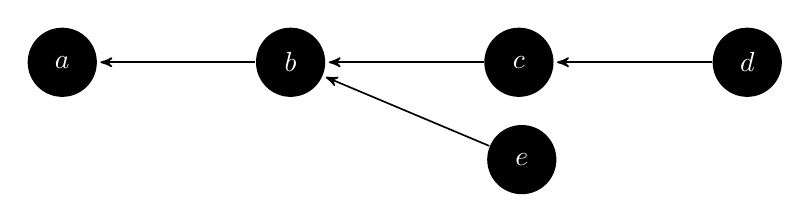
\begin{tikzpicture}[->,>=stealth',shorten >=1pt,auto,node distance=2cm,semithick]
	\tikzstyle{every state}=[fill=black,draw=none,text=white]

	\node[state] (A) {$a$};
	\node[state] (B) [right = of A] {$b$};
	\node[state] (C) [right = of B] {$c$};
	\node[state] (D) [right = of C] {$d$};
	\node[state] (E) [below right = 0.6 and 2.3 of B] {$e$};

	\path (B) edge (A);
        \path (C) edge (B);
        \path (D) edge (C);
        \path (E) edge (B);
\end{tikzpicture}
\end{document}